\documentclass[preprint,12pt]{elsarticle}
\usepackage{amsmath,amssymb,graphicx,booktabs,makecell}
\usepackage[hidelinks]{hyperref}
\renewcommand{\thetable}{S\arabic{table}}
\renewcommand{\thefigure}{S\arabic{figure}}
\journal{Meta-Radiology}

\begin{document}
\begin{frontmatter}
\title{Supplementary material}
\end{frontmatter}

\section*{S1. Validation before the full runs}
Each check was run before any full run, and the full runs used only the settings it fixed (Table~\ref{tab:validation}).

\begin{table}[!htbp]
\centering
\caption{Validation checks and the settings they fixed.}
\label{tab:validation}
\small
\begin{tabular}{p{0.14\textwidth}p{0.45\textwidth}p{0.31\textwidth}}
\toprule
Check & Result & Setting fixed \\
\midrule
V1 & All four API models parsed 100\% of single-reader answers through OpenRouter. GPT-5 mini used 256 reasoning tokens at low effort and 2,304 at high effort on the same prompt. & Claude Haiku 4.5 retained; GPT-5 mini at low effort. \\
V2 & Single-reader accuracy relative to the original image, over 10 model-by-data-set cells: CLAHE $-$0.0 percentage points on average (range $-$6 to $+$14), grayscale inversion $-$6.6 ($-$12 to $+$2), 256 pixels $-$1.0, 128 pixels $-$5.6. & Inversion exceeded the 5-point limit and was replaced by gamma 0.7: readers 4--6 of the rendering panel saw gamma 0.7, readers 7--9 CLAHE. \\
V3 & With four images per prompt (the query and three references), parsing was 100\%. A CLIP cosine threshold of 0.95 removed about 32 ordinary similar cases per query, because radiographs of different patients reach cosines of 0.91--0.95; a perceptual hash alone missed the same CT level and the same patient's chest radiograph (cosine 0.99). & References excluded if SHA-256 identical, within Hamming distance 8 of the 64-bit perceptual hash, or at CLIP cosine of at least 0.98. \\
V4 & SLAKE-target: 335 eligible questions, 250 sampled; in 20 inspected cases the target box covered the queried organ or lesion and the control box did not overlap it and lay within the body. SLAKE-pairs: 200 pairs over 104 question templates. & Used as built. \\
V5 & Findings reports had a median of 72--77 words (maximum 109); answer parsing 100\%. & Used as built. \\
V6 & With option-letter readout, the LLaVA family put 96--100\% of the probability on ``A'' regardless of the image. Pooled accuracy on 100 items (50 each from VQA-RAD and SLAKE): MedGemma 84\%, HuatuoGPT-Vision 79\%, Qwen3-VL 78\%, Qwen2-VL 74\%, LLaVA-1.5 55\%, LLaVA-Med 53\%. & Yes/no items read from the ``yes''/``no'' tokens; LLaVA-Med excluded by the 55\% rule. \\
Throughput & Qwen 3.8 Flash used 250--6,400 reasoning tokens and 6--77 s per call. & Qwen 3.8 Flash ran the original-image, graded-evidence, generic-panel and rendering conditions only. \\
\bottomrule
\end{tabular}
\end{table}

\section*{S2. Run record}
Claude Haiku 4.5 declined to answer for part of the gray-image prompts. Declined answers counted as wrong, the abstention rate is reported for each condition, and the error correlation on answered items is reported as a sensitivity analysis. The output-quality stop that ends a run when more than 15\% of answers cannot be parsed was designed to catch configuration errors and was turned off for the gray-image conditions. Each perceiver wrote its findings reports once for each image and slot before any reasoner read a report (12,906 reports; median length 75 to 90 words by perceiver, maximum 118 to 127). After each model finished, every condition was run again to fill episodes lost to transient errors; calls already made were read from the cache.

\section*{S3. Detailed results}
% Generated by experiments/radiology_numbers.py. Do not edit by hand.

\begin{table}[!htbp]
\centering
\scriptsize
\setlength{\tabcolsep}{4pt}
\caption{Reading panels with the original images. Accuracy with item bootstrap 95\% CI; pp, percentage points; round 0, the independent answers before discussion.}
\begin{tabular}{llcccc}
\toprule
\makecell{Set} & \makecell{Model} & \makecell{n} & \makecell{Single (\%)} & \makecell{Mean panel\\reader (\%)} & \makecell{Panel 9 (\%)} \\
\midrule
VQA-RAD & GPT-5 mini & 250 & \makecell{72.0\\{}[66.4, 77.2]} & \makecell{71.3\\{}[66.3, 76.2]} & \makecell{69.2\\{}[63.2, 74.8]} \\
VQA-RAD & Gemini 3.7 Flash & 250 & \makecell{81.2\\{}[76.4, 86.0]} & \makecell{81.3\\{}[76.9, 85.4]} & \makecell{82.4\\{}[77.2, 86.8]} \\
VQA-RAD & Claude Haiku 4.5 & 250 & \makecell{60.8\\{}[54.4, 66.8]} & \makecell{65.9\\{}[61.0, 71.0]} & \makecell{64.8\\{}[58.8, 70.8]} \\
VQA-RAD & Qwen 3.8 Flash & 250 & \makecell{69.6\\{}[64.0, 75.2]} & \makecell{79.9\\{}[76.3, 83.3]} & \makecell{83.2\\{}[78.4, 87.6]} \\
SLAKE & GPT-5 mini & 250 & \makecell{80.8\\{}[76.0, 85.6]} & \makecell{79.8\\{}[75.4, 84.3]} & \makecell{78.4\\{}[73.2, 83.6]} \\
SLAKE & Gemini 3.7 Flash & 250 & \makecell{91.2\\{}[87.6, 94.4]} & \makecell{89.9\\{}[86.7, 93.1]} & \makecell{90.0\\{}[86.4, 93.6]} \\
SLAKE & Claude Haiku 4.5 & 250 & \makecell{72.4\\{}[67.2, 78.0]} & \makecell{72.3\\{}[67.4, 77.0]} & \makecell{72.4\\{}[66.8, 78.0]} \\
SLAKE & Qwen 3.8 Flash & 250 & \makecell{76.4\\{}[70.8, 81.2]} & \makecell{83.3\\{}[79.9, 87.0]} & \makecell{84.4\\{}[80.0, 89.2]} \\
MedXpertQA-MM & GPT-5 mini & 250 & \makecell{54.8\\{}[48.8, 60.4]} & \makecell{53.2\\{}[48.1, 58.4]} & \makecell{55.6\\{}[49.6, 61.6]} \\
MedXpertQA-MM & Gemini 3.7 Flash & 250 & \makecell{84.4\\{}[79.6, 88.8]} & \makecell{83.3\\{}[79.2, 87.2]} & \makecell{83.6\\{}[78.8, 88.4]} \\
MedXpertQA-MM & Claude Haiku 4.5 & 250 & \makecell{33.2\\{}[27.6, 38.8]} & \makecell{30.8\\{}[25.4, 36.1]} & \makecell{30.4\\{}[24.4, 36.0]} \\
MedXpertQA-MM & Qwen 3.8 Flash & 250 & \makecell{43.6\\{}[37.6, 49.6]} & \makecell{46.7\\{}[41.9, 51.8]} & \makecell{49.2\\{}[43.2, 55.2]} \\
\bottomrule
\end{tabular}
\end{table}

\begin{table}[!htbp]
\centering
\scriptsize
\setlength{\tabcolsep}{4pt}
\caption{Reading panels with the original images (continued).}
\begin{tabular}{llcccc}
\toprule
\makecell{Set} & \makecell{Model} & \makecell{Discussion 9\\(\%)} & \makecell{Panel 9 $-$\\single (pp)} & \makecell{Mean panel\\reader $-$\\single (pp)} & \makecell{Panel 9 $-$\\its mean\\reader (pp)} \\
\midrule
VQA-RAD & GPT-5 mini & \makecell{70.0\\{}[64.0, 75.6]} & \makecell{$-$2.8\\{}[$-$6.4, +0.8]} & \makecell{$-$0.7\\{}[$-$3.5, +2.2]} & \makecell{$-$2.1\\{}[$-$4.0, $-$0.4]} \\
VQA-RAD & Gemini 3.7 Flash & \makecell{81.2\\{}[76.0, 86.0]} & \makecell{+1.2\\{}[$-$2.4, +4.8]} & \makecell{+0.1\\{}[$-$2.7, +2.7]} & \makecell{+1.1\\{}[$-$0.5, +2.7]} \\
VQA-RAD & Claude Haiku 4.5 & \makecell{66.4\\{}[60.4, 72.4]} & \makecell{+4.0\\{}[$-$0.8, +8.8]} & \makecell{+5.1\\{}[+1.0, +9.1]} & \makecell{$-$1.1\\{}[$-$3.1, +0.8]} \\
VQA-RAD & Qwen 3.8 Flash & \makecell{80.4\\{}[75.6, 85.2]} & \makecell{+13.6\\{}[+7.6, +19.6]} & \makecell{+10.3\\{}[+5.2, +15.5]} & \makecell{+3.3\\{}[+0.8, +5.8]} \\
SLAKE & GPT-5 mini & \makecell{80.8\\{}[75.6, 85.6]} & \makecell{$-$2.4\\{}[$-$5.2, +0.4]} & \makecell{$-$1.0\\{}[$-$3.5, +1.3]} & \makecell{$-$1.4\\{}[$-$2.9, +0.0]} \\
SLAKE & Gemini 3.7 Flash & \makecell{89.2\\{}[85.2, 93.2]} & \makecell{$-$1.2\\{}[$-$3.2, +0.4]} & \makecell{$-$1.3\\{}[$-$2.8, +0.1]} & \makecell{+0.1\\{}[$-$1.0, +1.3]} \\
SLAKE & Claude Haiku 4.5 & \makecell{74.4\\{}[69.2, 79.6]} & \makecell{+0.0\\{}[$-$4.4, +4.4]} & \makecell{$-$0.1\\{}[$-$3.8, +3.6]} & \makecell{+0.1\\{}[$-$1.6, +1.7]} \\
SLAKE & Qwen 3.8 Flash & \makecell{90.4\\{}[86.8, 94.0]} & \makecell{+8.0\\{}[+4.0, +12.4]} & \makecell{+6.9\\{}[+3.5, +10.6]} & \makecell{+1.1\\{}[$-$0.8, +2.9]} \\
MedXpertQA-MM & GPT-5 mini & \makecell{58.4\\{}[52.4, 64.4]} & \makecell{+0.8\\{}[$-$3.6, +5.6]} & \makecell{$-$1.6\\{}[$-$5.2, +2.4]} & \makecell{+2.4\\{}[+0.1, +4.6]} \\
MedXpertQA-MM & Gemini 3.7 Flash & \makecell{82.4\\{}[77.6, 87.2]} & \makecell{$-$0.8\\{}[$-$4.0, +2.4]} & \makecell{$-$1.1\\{}[$-$3.5, +1.2]} & \makecell{+0.3\\{}[$-$1.4, +2.0]} \\
MedXpertQA-MM & Claude Haiku 4.5 & \makecell{30.0\\{}[24.4, 36.0]} & \makecell{$-$2.8\\{}[$-$6.0, +0.4]} & \makecell{$-$2.4\\{}[$-$5.4, +0.5]} & \makecell{$-$0.4\\{}[$-$1.9, +1.1]} \\
MedXpertQA-MM & Qwen 3.8 Flash & \makecell{52.4\\{}[45.6, 58.8]} & \makecell{+5.6\\{}[+0.4, +11.2]} & \makecell{+3.1\\{}[$-$1.5, +7.6]} & \makecell{+2.5\\{}[+0.0, +4.9]} \\
\bottomrule
\end{tabular}
\end{table}

\begin{table}[!htbp]
\centering
\scriptsize
\setlength{\tabcolsep}{4pt}
\caption{Reading panels with the original images (continued).}
\begin{tabular}{llcccc}
\toprule
\makecell{Set} & \makecell{Model} & \makecell{Discussion 9\\$-$ single\\(pp)} & \makecell{$\phi$ round 0} & \makecell{$N_{\mathrm{eff}}$} & \makecell{Unanimous r0\\(\%)} \\
\midrule
VQA-RAD & GPT-5 mini & \makecell{$-$2.0\\{}[$-$5.6, +1.6]} & \makecell{0.752\\{}[0.697, 0.801]} & 1.28 & 74.4 \\
VQA-RAD & Gemini 3.7 Flash & \makecell{+0.0\\{}[$-$3.6, +3.6]} & \makecell{0.725\\{}[0.653, 0.785]} & 1.32 & 76.0 \\
VQA-RAD & Claude Haiku 4.5 & \makecell{+5.6\\{}[+0.8, +10.8]} & \makecell{0.731\\{}[0.678, 0.781]} & 1.31 & 68.0 \\
VQA-RAD & Qwen 3.8 Flash & \makecell{+10.8\\{}[+5.2, +16.4]} & \makecell{0.439\\{}[0.369, 0.501]} & 1.99 & 54.8 \\
SLAKE & GPT-5 mini & \makecell{+0.0\\{}[$-$2.8, +2.8]} & \makecell{0.785\\{}[0.729, 0.844]} & 1.24 & 82.0 \\
SLAKE & Gemini 3.7 Flash & \makecell{$-$2.0\\{}[$-$4.4, +0.0]} & \makecell{0.785\\{}[0.696, 0.859]} & 1.24 & 90.4 \\
SLAKE & Claude Haiku 4.5 & \makecell{+2.0\\{}[$-$2.0, +6.0]} & \makecell{0.775\\{}[0.723, 0.821]} & 1.25 & 75.6 \\
SLAKE & Qwen 3.8 Flash & \makecell{+14.0\\{}[+9.2, +18.8]} & \makecell{0.529\\{}[0.448, 0.597]} & 1.72 & 65.6 \\
MedXpertQA-MM & GPT-5 mini & \makecell{+3.6\\{}[$-$0.8, +8.0]} & \makecell{0.685\\{}[0.636, 0.735]} & 1.39 & 52.4 \\
MedXpertQA-MM & Gemini 3.7 Flash & \makecell{$-$2.0\\{}[$-$5.2, +0.8]} & \makecell{0.749\\{}[0.669, 0.817]} & 1.29 & 82.4 \\
MedXpertQA-MM & Claude Haiku 4.5 & \makecell{$-$3.2\\{}[$-$6.8, +0.4]} & \makecell{0.836\\{}[0.790, 0.882]} & 1.17 & 71.6 \\
MedXpertQA-MM & Qwen 3.8 Flash & \makecell{+8.8\\{}[+3.6, +14.4]} & \makecell{0.647\\{}[0.591, 0.701]} & 1.46 & 41.2 \\
\bottomrule
\end{tabular}
\end{table}

\begin{table}[!htbp]
\centering
\scriptsize
\setlength{\tabcolsep}{4pt}
\caption{Reading panels with the original images (continued).}
\begin{tabular}{llcccc}
\toprule
\makecell{Set} & \makecell{Model} & \makecell{Wrong if\\unanimous r0\\(\%)} & \makecell{$\phi$ final} & \makecell{Unanimous\\final (\%)} & \makecell{Wrong if\\unanimous\\final (\%)} \\
\midrule
VQA-RAD & GPT-5 mini & 20.4 & \makecell{1.000\\{}[1.000, 1.000]} & 100.0 & 30.0 \\
VQA-RAD & Gemini 3.7 Flash & 11.6 & \makecell{0.997\\{}[0.991, 1.000]} & 99.6 & 18.9 \\
VQA-RAD & Claude Haiku 4.5 & 25.9 & \makecell{0.996\\{}[0.990, 1.000]} & 99.2 & 33.5 \\
VQA-RAD & Qwen 3.8 Flash & 5.8 & \makecell{0.822\\{}[0.762, 0.874]} & 86.0 & 15.8 \\
SLAKE & GPT-5 mini & 12.2 & \makecell{0.995\\{}[0.984, 1.000]} & 99.6 & 18.9 \\
SLAKE & Gemini 3.7 Flash & 5.8 & \makecell{1.000\\{}[1.000, 1.000]} & 100.0 & 10.8 \\
SLAKE & Claude Haiku 4.5 & 22.2 & \makecell{1.000\\{}[1.000, 1.000]} & 100.0 & 25.6 \\
SLAKE & Qwen 3.8 Flash & 4.3 & \makecell{0.884\\{}[0.811, 0.940]} & 94.4 & 8.9 \\
MedXpertQA-MM & GPT-5 mini & 35.9 & \makecell{0.996\\{}[0.991, 1.000]} & 98.8 & 41.7 \\
MedXpertQA-MM & Gemini 3.7 Flash & 9.2 & \makecell{1.000\\{}[1.000, 1.000]} & 100.0 & 17.6 \\
MedXpertQA-MM & Claude Haiku 4.5 & 68.7 & \makecell{1.000\\{}[1.000, 1.000]} & 100.0 & 70.0 \\
MedXpertQA-MM & Qwen 3.8 Flash & 36.9 & \makecell{0.913\\{}[0.883, 0.941]} & 82.4 & 42.7 \\
\bottomrule
\end{tabular}
\end{table}

\begin{table}[!htbp]
\centering
\scriptsize
\setlength{\tabcolsep}{4pt}
\caption{Graded image evidence: single-reader accuracy (\%) and error correlation $\phi$ of the independent panel of 9 at each evidence level; paired differences between the original and the gray image.}
\begin{tabular}{llcccc}
\toprule
\makecell{Set} & \makecell{Model} & \makecell{Single $\le$1024} & \makecell{Single 256} & \makecell{Single 128} & \makecell{Single gray} \\
\midrule
VQA-RAD & GPT-5 mini & \makecell{72.0\\{}[66.4, 77.2]} & \makecell{74.0\\{}[68.8, 79.2]} & \makecell{72.8\\{}[67.2, 78.0]} & \makecell{60.8\\{}[54.8, 66.4]} \\
VQA-RAD & Gemini 3.7 Flash & \makecell{81.2\\{}[76.4, 86.0]} & \makecell{83.6\\{}[78.8, 88.0]} & \makecell{77.6\\{}[72.4, 82.4]} & \makecell{54.4\\{}[48.4, 60.4]} \\
VQA-RAD & Claude Haiku 4.5 & \makecell{60.8\\{}[54.4, 66.8]} & \makecell{63.2\\{}[57.2, 69.2]} & \makecell{65.2\\{}[59.2, 70.8]} & \makecell{46.8\\{}[40.8, 52.8]} \\
VQA-RAD & Qwen 3.8 Flash & \makecell{69.6\\{}[64.0, 75.2]} & \makecell{67.6\\{}[61.6, 73.2]} & \makecell{72.0\\{}[66.4, 77.6]} & \makecell{54.8\\{}[48.4, 60.8]} \\
SLAKE & GPT-5 mini & \makecell{80.8\\{}[76.0, 85.6]} & \makecell{78.8\\{}[73.6, 83.6]} & \makecell{75.2\\{}[70.0, 80.4]} & \makecell{54.4\\{}[48.4, 60.8]} \\
SLAKE & Gemini 3.7 Flash & \makecell{91.2\\{}[87.6, 94.4]} & \makecell{91.2\\{}[87.6, 94.8]} & \makecell{85.2\\{}[80.8, 89.2]} & \makecell{51.2\\{}[44.8, 57.6]} \\
SLAKE & Claude Haiku 4.5 & \makecell{72.4\\{}[67.2, 78.0]} & \makecell{73.6\\{}[68.0, 78.8]} & \makecell{70.0\\{}[64.4, 75.6]} & \makecell{38.8\\{}[32.8, 44.8]} \\
SLAKE & Qwen 3.8 Flash & \makecell{76.4\\{}[70.8, 81.2]} & \makecell{74.8\\{}[69.2, 80.8]} & \makecell{79.2\\{}[74.4, 84.0]} & \makecell{51.2\\{}[44.8, 57.2]} \\
MedXpertQA-MM & GPT-5 mini & \makecell{54.8\\{}[48.8, 60.4]} & \makecell{50.4\\{}[44.4, 56.8]} & \makecell{50.8\\{}[44.8, 56.8]} & \makecell{50.8\\{}[44.8, 56.4]} \\
MedXpertQA-MM & Gemini 3.7 Flash & \makecell{84.4\\{}[79.6, 88.8]} & \makecell{80.4\\{}[75.2, 85.2]} & \makecell{78.4\\{}[73.2, 83.2]} & \makecell{66.4\\{}[60.8, 71.6]} \\
MedXpertQA-MM & Claude Haiku 4.5 & \makecell{33.2\\{}[27.6, 38.8]} & \makecell{32.0\\{}[26.4, 37.6]} & \makecell{32.0\\{}[26.4, 37.6]} & \makecell{29.6\\{}[24.0, 35.2]} \\
MedXpertQA-MM & Qwen 3.8 Flash & \makecell{43.6\\{}[37.6, 49.6]} & \makecell{40.8\\{}[34.8, 47.2]} & \makecell{43.2\\{}[37.2, 49.6]} & \makecell{41.6\\{}[35.6, 47.6]} \\
\bottomrule
\end{tabular}
\end{table}

\begin{table}[!htbp]
\centering
\scriptsize
\setlength{\tabcolsep}{4pt}
\caption{Graded image evidence (continued).}
\begin{tabular}{llcccc}
\toprule
\makecell{Set} & \makecell{Model} & \makecell{$\phi$ $\le$1024} & \makecell{$\phi$ 256} & \makecell{$\phi$ 128} & \makecell{$\phi$ gray} \\
\midrule
VQA-RAD & GPT-5 mini & \makecell{0.752\\{}[0.697, 0.801]} & \makecell{0.694\\{}[0.636, 0.751]} & \makecell{0.644\\{}[0.586, 0.703]} & \makecell{0.742\\{}[0.689, 0.789]} \\
VQA-RAD & Gemini 3.7 Flash & \makecell{0.725\\{}[0.653, 0.785]} & \makecell{0.726\\{}[0.646, 0.793]} & \makecell{0.749\\{}[0.698, 0.804]} & \makecell{0.922\\{}[0.889, 0.951]} \\
VQA-RAD & Claude Haiku 4.5 & \makecell{0.731\\{}[0.678, 0.781]} & \makecell{0.706\\{}[0.651, 0.756]} & \makecell{0.591\\{}[0.539, 0.650]} & \makecell{0.876\\{}[0.840, 0.911]} \\
VQA-RAD & Qwen 3.8 Flash & \makecell{0.439\\{}[0.369, 0.501]} & \makecell{0.442\\{}[0.377, 0.501]} & \makecell{0.480\\{}[0.415, 0.541]} & \makecell{0.841\\{}[0.805, 0.879]} \\
SLAKE & GPT-5 mini & \makecell{0.785\\{}[0.729, 0.844]} & \makecell{0.792\\{}[0.741, 0.845]} & \makecell{0.709\\{}[0.645, 0.761]} & \makecell{0.802\\{}[0.755, 0.845]} \\
SLAKE & Gemini 3.7 Flash & \makecell{0.785\\{}[0.696, 0.859]} & \makecell{0.803\\{}[0.716, 0.869]} & \makecell{0.820\\{}[0.753, 0.872]} & \makecell{0.982\\{}[0.968, 0.994]} \\
SLAKE & Claude Haiku 4.5 & \makecell{0.775\\{}[0.723, 0.821]} & \makecell{0.752\\{}[0.695, 0.811]} & \makecell{0.718\\{}[0.664, 0.768]} & \makecell{0.879\\{}[0.841, 0.915]} \\
SLAKE & Qwen 3.8 Flash & \makecell{0.529\\{}[0.448, 0.597]} & \makecell{0.547\\{}[0.479, 0.607]} & \makecell{0.490\\{}[0.408, 0.560]} & \makecell{0.831\\{}[0.788, 0.866]} \\
MedXpertQA-MM & GPT-5 mini & \makecell{0.685\\{}[0.636, 0.735]} & \makecell{0.690\\{}[0.637, 0.739]} & \makecell{0.700\\{}[0.652, 0.752]} & \makecell{0.730\\{}[0.679, 0.780]} \\
MedXpertQA-MM & Gemini 3.7 Flash & \makecell{0.749\\{}[0.669, 0.817]} & \makecell{0.762\\{}[0.698, 0.823]} & \makecell{0.784\\{}[0.715, 0.841]} & \makecell{0.799\\{}[0.748, 0.844]} \\
MedXpertQA-MM & Claude Haiku 4.5 & \makecell{0.836\\{}[0.790, 0.882]} & \makecell{0.821\\{}[0.776, 0.868]} & \makecell{0.840\\{}[0.795, 0.881]} & \makecell{0.818\\{}[0.765, 0.861]} \\
MedXpertQA-MM & Qwen 3.8 Flash & \makecell{0.647\\{}[0.591, 0.701]} & \makecell{0.630\\{}[0.573, 0.688]} & \makecell{0.609\\{}[0.556, 0.667]} & \makecell{0.656\\{}[0.602, 0.709]} \\
\bottomrule
\end{tabular}
\end{table}

\begin{table}[!htbp]
\centering
\scriptsize
\setlength{\tabcolsep}{4pt}
\caption{Graded image evidence (continued).}
\begin{tabular}{llcccc}
\toprule
\makecell{Set} & \makecell{Model} & \makecell{Single real\\$-$ gray (pp)} & \makecell{Panel 9 real\\$-$ gray (pp)} & \makecell{Abstention\\gray (\%)} & \makecell{$\phi$ gray,\\answered\\only} \\
\midrule
VQA-RAD & GPT-5 mini & \makecell{+11.2\\{}[+4.0, +18.4]} & \makecell{+7.6\\{}[+0.4, +14.8]} & – & – \\
VQA-RAD & Gemini 3.7 Flash & \makecell{+26.8\\{}[+18.8, +35.2]} & \makecell{+28.4\\{}[+20.8, +36.8]} & – & – \\
VQA-RAD & Claude Haiku 4.5 & \makecell{+14.0\\{}[+6.0, +22.0]} & \makecell{+10.4\\{}[+2.8, +18.4]} & 10.4 & \makecell{0.963\\{}[0.942, 0.982]} \\
VQA-RAD & Qwen 3.8 Flash & \makecell{+14.8\\{}[+6.4, +23.2]} & \makecell{+26.0\\{}[+18.4, +34.0]} & 0.1 & – \\
SLAKE & GPT-5 mini & \makecell{+26.4\\{}[+18.8, +33.2]} & \makecell{+25.6\\{}[+18.0, +33.2]} & – & – \\
SLAKE & Gemini 3.7 Flash & \makecell{+40.0\\{}[+33.2, +46.8]} & \makecell{+39.2\\{}[+32.4, +46.0]} & – & – \\
SLAKE & Claude Haiku 4.5 & \makecell{+33.6\\{}[+24.0, +42.8]} & \makecell{+28.4\\{}[+19.6, +37.2]} & 4.3 & \makecell{0.931\\{}[0.901, 0.956]} \\
SLAKE & Qwen 3.8 Flash & \makecell{+25.2\\{}[+16.4, +33.6]} & \makecell{+33.6\\{}[+25.6, +42.0]} & – & – \\
MedXpertQA-MM & GPT-5 mini & \makecell{+4.0\\{}[$-$2.0, +10.0]} & \makecell{+6.8\\{}[+1.6, +12.0]} & – & – \\
MedXpertQA-MM & Gemini 3.7 Flash & \makecell{+18.0\\{}[+12.0, +23.6]} & \makecell{+17.6\\{}[+12.0, +23.6]} & – & – \\
MedXpertQA-MM & Claude Haiku 4.5 & \makecell{+3.6\\{}[$-$0.4, +8.0]} & \makecell{+0.0\\{}[$-$4.4, +4.4]} & 14.8 & \makecell{0.852\\{}[0.803, 0.891]} \\
MedXpertQA-MM & Qwen 3.8 Flash & \makecell{+2.0\\{}[$-$4.4, +8.0]} & \makecell{+9.6\\{}[+4.8, +14.8]} & 0.5 & – \\
\bottomrule
\end{tabular}
\end{table}

\begin{table}[!htbp]
\centering
\scriptsize
\setlength{\tabcolsep}{4pt}
\caption{Reader answers of the independent panel of 9 cross-tabulated by correctness with the original and with the gray image (\% of answers), and consensus errors (at least 7 of 9 readers wrong) whose majority answer equals the gray-image majority.}
\begin{tabular}{llcccc}
\toprule
\makecell{Set} & \makecell{Model} & \makecell{Right with\\and without\\image} & \makecell{Right only\\with image} & \makecell{Wrong only\\with image} & \makecell{Wrong with\\and without\\image} \\
\midrule
VQA-RAD & GPT-5 mini & 47.2 & 24.1 & 12.0 & 16.7 \\
VQA-RAD & Gemini 3.7 Flash & 44.0 & 37.3 & 10.4 & 8.3 \\
VQA-RAD & Claude Haiku 4.5 & 36.6 & 29.3 & 13.6 & 20.5 \\
VQA-RAD & Qwen 3.8 Flash & 46.0 & 33.9 & 10.8 & 9.3 \\
SLAKE & GPT-5 mini & 43.5 & 36.3 & 9.5 & 10.7 \\
SLAKE & Gemini 3.7 Flash & 46.7 & 43.2 & 4.4 & 5.8 \\
SLAKE & Claude Haiku 4.5 & 25.9 & 46.4 & 15.8 & 11.9 \\
SLAKE & Qwen 3.8 Flash & 38.5 & 44.8 & 12.0 & 4.7 \\
MedXpertQA-MM & GPT-5 mini & 39.7 & 13.5 & 7.9 & 38.9 \\
MedXpertQA-MM & Gemini 3.7 Flash & 61.0 & 22.3 & 4.4 & 12.3 \\
MedXpertQA-MM & Claude Haiku 4.5 & 22.7 & 8.1 & 5.2 & 64.0 \\
MedXpertQA-MM & Qwen 3.8 Flash & 32.9 & 13.8 & 7.0 & 46.4 \\
\bottomrule
\end{tabular}
\end{table}

\begin{table}[!htbp]
\centering
\scriptsize
\setlength{\tabcolsep}{4pt}
\caption{Reader answers of the independent panel of 9 cross-tabulated by correctness with the original and with the gray image (\% of answers), and consensus errors (at least 7 of 9 readers wrong) whose majority answer equals the gray-image majority (continued).}
\begin{tabular}{llcc}
\toprule
\makecell{Set} & \makecell{Model} & \makecell{Consensus\\errors (n)} & \makecell{Consensus\\errors =\\gray-image\\majority (\%)} \\
\midrule
VQA-RAD & GPT-5 mini & 57 & \makecell{54.4\\{}[42.1, 66.7]} \\
VQA-RAD & Gemini 3.7 Flash & 35 & \makecell{42.9\\{}[25.7, 60.0]} \\
VQA-RAD & Claude Haiku 4.5 & 70 & \makecell{54.3\\{}[42.9, 65.7]} \\
VQA-RAD & Qwen 3.8 Flash & 18 & \makecell{44.4\\{}[22.2, 66.7]} \\
SLAKE & GPT-5 mini & 42 & \makecell{57.1\\{}[42.9, 71.4]} \\
SLAKE & Gemini 3.7 Flash & 19 & \makecell{57.9\\{}[36.8, 78.9]} \\
SLAKE & Claude Haiku 4.5 & 56 & \makecell{33.9\\{}[21.4, 46.4]} \\
SLAKE & Qwen 3.8 Flash & 21 & \makecell{14.3\\{}[0.0, 28.6]} \\
MedXpertQA-MM & GPT-5 mini & 95 & \makecell{64.2\\{}[54.7, 72.7]} \\
MedXpertQA-MM & Gemini 3.7 Flash & 31 & \makecell{74.2\\{}[58.1, 90.3]} \\
MedXpertQA-MM & Claude Haiku 4.5 & 163 & \makecell{71.2\\{}[64.4, 77.9]} \\
MedXpertQA-MM & Qwen 3.8 Flash & 105 & \makecell{76.2\\{}[67.6, 83.8]} \\
\bottomrule
\end{tabular}
\end{table}

\begin{table}[!htbp]
\centering
\scriptsize
\setlength{\tabcolsep}{4pt}
\caption{Region occlusion on SLAKE-target: share of answers changed by covering the target box or an equal-size control box, and region dependence (target minus control).}
\begin{tabular}{llcccc}
\toprule
\makecell{Model} & \makecell{Arm} & \makecell{Target flip\\(\%)} & \makecell{Control flip\\(\%)} & \makecell{Region\\dependence\\(pp)} & \makecell{Single\\target flip\\(\%)} \\
\midrule
GPT-5 mini & API, panel readers & \makecell{23.5\\{}[19.7, 27.6]} & \makecell{6.4\\{}[4.7, 8.4]} & \makecell{+17.1\\{}[+13.2, +21.2]} & \makecell{26.4\\{}[20.8, 32.0]} \\
Gemini 3.7 Flash & API, panel readers & \makecell{36.4\\{}[31.6, 41.4]} & \makecell{3.6\\{}[2.4, 4.9]} & \makecell{+32.9\\{}[+28.2, +38.0]} & \makecell{36.8\\{}[30.8, 42.8]} \\
Claude Haiku 4.5 & API, panel readers & \makecell{10.7\\{}[8.2, 13.6]} & \makecell{7.5\\{}[5.5, 9.6]} & \makecell{+3.2\\{}[+0.8, +5.7]} & \makecell{8.4\\{}[5.2, 12.0]} \\
HuatuoGPT-Vision 7B & open weight & \makecell{28.0\\{}[22.4, 34.0]} & \makecell{6.4\\{}[3.6, 9.6]} & \makecell{+21.6\\{}[+15.6, +28.0]} &  \\
LLaVA-1.5 7B & open weight & \makecell{12.8\\{}[8.8, 17.2]} & \makecell{10.4\\{}[6.8, 14.4]} & \makecell{+2.4\\{}[$-$2.0, +6.8]} &  \\
MedGemma 4B & open weight & \makecell{13.2\\{}[9.2, 17.6]} & \makecell{1.6\\{}[0.4, 3.2]} & \makecell{+11.6\\{}[+7.6, +15.6]} &  \\
Qwen2-VL 7B & open weight & \makecell{11.2\\{}[7.6, 15.2]} & \makecell{4.8\\{}[2.4, 7.6]} & \makecell{+6.4\\{}[+2.0, +10.4]} &  \\
Qwen3-VL 8B & open weight & \makecell{23.6\\{}[18.4, 28.8]} & \makecell{3.6\\{}[1.6, 6.0]} & \makecell{+20.0\\{}[+14.4, +26.0]} &  \\
\bottomrule
\end{tabular}
\end{table}

\begin{table}[!htbp]
\centering
\scriptsize
\setlength{\tabcolsep}{4pt}
\caption{Region occlusion on SLAKE-target (continued).}
\begin{tabular}{llcc}
\toprule
\makecell{Model} & \makecell{Arm} & \makecell{Single\\control flip\\(\%)} & \makecell{Single\\region\\dependence\\(pp)} \\
\midrule
GPT-5 mini & API, panel readers & \makecell{8.4\\{}[5.2, 12.0]} & \makecell{+18.0\\{}[+11.6, +24.8]} \\
Gemini 3.7 Flash & API, panel readers & \makecell{2.8\\{}[1.2, 4.8]} & \makecell{+34.0\\{}[+28.0, +40.4]} \\
Claude Haiku 4.5 & API, panel readers & \makecell{6.4\\{}[3.6, 9.2]} & \makecell{+2.0\\{}[$-$1.6, +5.2]} \\
HuatuoGPT-Vision 7B & open weight &  &  \\
LLaVA-1.5 7B & open weight &  &  \\
MedGemma 4B & open weight &  &  \\
Qwen2-VL 7B & open weight &  &  \\
Qwen3-VL 8B & open weight &  &  \\
\bottomrule
\end{tabular}
\end{table}

\begin{table}[!htbp]
\centering
\scriptsize
\setlength{\tabcolsep}{4pt}
\caption{Same question, different image (SLAKE-pairs, 200 pairs with opposite reference answers).}
\begin{tabular}{lcccc}
\toprule
\makecell{Model} & \makecell{Single: both\\correct (\%)} & \makecell{Single:\\answers\\differ (\%)} & \makecell{Panel 9:\\both correct\\(\%)} & \makecell{Panel 9:\\answers\\differ (\%)} \\
\midrule
GPT-5 mini & \makecell{59.0\\{}[52.0, 65.5]} & \makecell{62.0\\{}[55.5, 68.5]} & \makecell{62.0\\{}[55.5, 68.5]} & \makecell{65.0\\{}[58.0, 71.0]} \\
Gemini 3.7 Flash & \makecell{74.0\\{}[67.5, 80.0]} & \makecell{75.0\\{}[69.0, 81.0]} & \makecell{74.5\\{}[68.0, 80.5]} & \makecell{75.5\\{}[69.0, 81.5]} \\
Claude Haiku 4.5 & \makecell{38.5\\{}[31.5, 45.0]} & \makecell{42.5\\{}[35.5, 49.5]} & \makecell{42.5\\{}[35.5, 49.0]} & \makecell{46.0\\{}[39.0, 52.5]} \\
HuatuoGPT-Vision 7B (open weight) & \makecell{48.5\\{}[41.5, 55.5]} & \makecell{53.0\\{}[46.0, 60.0]} &  &  \\
LLaVA-1.5 7B (open weight) & \makecell{31.5\\{}[25.5, 38.0]} & \makecell{39.5\\{}[33.0, 46.5]} &  &  \\
MedGemma 4B (open weight) & \makecell{62.5\\{}[56.0, 68.5]} & \makecell{63.5\\{}[57.0, 69.5]} &  &  \\
Qwen2-VL 7B (open weight) & \makecell{49.5\\{}[42.5, 56.0]} & \makecell{53.5\\{}[46.5, 60.0]} &  &  \\
Qwen3-VL 8B (open weight) & \makecell{53.5\\{}[46.5, 60.5]} & \makecell{56.5\\{}[49.5, 63.0]} &  &  \\
\bottomrule
\end{tabular}
\end{table}

\begin{table}[!htbp]
\centering
\scriptsize
\setlength{\tabcolsep}{4pt}
\caption{Same question, different image (SLAKE-pairs, 200 pairs with opposite reference answers) (continued).}
\begin{tabular}{lc}
\toprule
\makecell{Model} & \makecell{Readers:\\answers\\differ (\%)} \\
\midrule
GPT-5 mini & \makecell{66.0\\{}[60.4, 71.2]} \\
Gemini 3.7 Flash & \makecell{75.9\\{}[70.1, 81.4]} \\
Claude Haiku 4.5 & \makecell{45.3\\{}[39.2, 51.3]} \\
HuatuoGPT-Vision 7B (open weight) &  \\
LLaVA-1.5 7B (open weight) &  \\
MedGemma 4B (open weight) &  \\
Qwen2-VL 7B (open weight) &  \\
Qwen3-VL 8B (open weight) &  \\
\bottomrule
\end{tabular}
\end{table}

\begin{table}[!htbp]
\centering
\scriptsize
\setlength{\tabcolsep}{4pt}
\caption{Discussion: readers correct in round 0 who ended the discussion wrong, by whether their round-0 answer differed from their gray-image answer and by round-0 position.}
\begin{tabular}{llcccc}
\toprule
\makecell{Set} & \makecell{Model} & \makecell{Abandoned,\\from image\\(\%)} & \makecell{Abandoned,\\same as\\prior (\%)} & \makecell{Difference\\(pp)} & \makecell{Abandoned,\\in minority\\(\%)} \\
\midrule
VQA-RAD & GPT-5 mini & \makecell{9.8\\{}[5.5, 14.9]} & \makecell{4.6\\{}[2.3, 7.4]} & \makecell{+5.1\\{}[+0.4, +10.4]} & \makecell{72.3\\{}[55.2, 88.9]} \\
VQA-RAD & Gemini 3.7 Flash & \makecell{3.7\\{}[1.4, 6.2]} & \makecell{3.4\\{}[1.6, 5.7]} & \makecell{+0.3\\{}[$-$2.9, +3.3]} & \makecell{100.0\\{}[100.0, 100.0]} \\
VQA-RAD & Claude Haiku 4.5 & \makecell{7.1\\{}[3.9, 11.0]} & \makecell{5.7\\{}[3.1, 8.9]} & \makecell{+1.4\\{}[$-$2.9, +5.9]} & \makecell{75.0\\{}[59.2, 89.7]} \\
VQA-RAD & Qwen 3.8 Flash & \makecell{12.5\\{}[7.8, 17.7]} & \makecell{6.6\\{}[3.8, 9.8]} & \makecell{+5.9\\{}[+0.6, +11.5]} & \makecell{54.1\\{}[37.4, 70.6]} \\
SLAKE & GPT-5 mini & \makecell{4.5\\{}[2.1, 7.3]} & \makecell{1.9\\{}[0.8, 3.3]} & \makecell{+2.6\\{}[+0.3, +5.2]} & \makecell{56.1\\{}[34.9, 78.8]} \\
SLAKE & Gemini 3.7 Flash & \makecell{2.9\\{}[0.7, 5.3]} & \makecell{1.4\\{}[0.3, 2.9]} & \makecell{+1.5\\{}[$-$1.1, +4.2]} & \makecell{71.4\\{}[41.2, 100.0]} \\
SLAKE & Claude Haiku 4.5 & \makecell{4.0\\{}[1.9, 6.7]} & \makecell{3.4\\{}[1.1, 6.4]} & \makecell{+0.6\\{}[$-$3.3, +4.1]} & \makecell{62.5\\{}[41.4, 83.0]} \\
SLAKE & Qwen 3.8 Flash & \makecell{4.2\\{}[2.0, 6.9]} & \makecell{2.8\\{}[1.3, 4.6]} & \makecell{+1.4\\{}[$-$1.4, +4.6]} & \makecell{41.5\\{}[23.7, 61.2]} \\
MedXpertQA-MM & GPT-5 mini & \makecell{18.1\\{}[11.5, 26.1]} & \makecell{2.7\\{}[1.4, 4.3]} & \makecell{+15.4\\{}[+9.6, +23.1]} & \makecell{68.5\\{}[52.6, 85.3]} \\
MedXpertQA-MM & Gemini 3.7 Flash & \makecell{7.2\\{}[3.7, 11.6]} & \makecell{2.6\\{}[1.2, 4.5]} & \makecell{+4.6\\{}[+0.8, +9.0]} & \makecell{71.7\\{}[48.0, 93.9]} \\
MedXpertQA-MM & Claude Haiku 4.5 & \makecell{23.6\\{}[12.8, 36.3]} & \makecell{6.3\\{}[2.9, 11.1]} & \makecell{+17.4\\{}[+6.4, +29.7]} & \makecell{83.9\\{}[67.3, 100.0]} \\
MedXpertQA-MM & Qwen 3.8 Flash & \makecell{18.1\\{}[12.3, 25.1]} & \makecell{5.4\\{}[2.9, 8.5]} & \makecell{+12.7\\{}[+6.6, +19.8]} & \makecell{62.2\\{}[48.6, 76.7]} \\
\bottomrule
\end{tabular}
\end{table}

\begin{table}[!htbp]
\centering
\scriptsize
\setlength{\tabcolsep}{4pt}
\caption{Discussion (continued).}
\begin{tabular}{llcccc}
\toprule
\makecell{Set} & \makecell{Model} & \makecell{Abandoned,\\in majority\\(\%)} & \makecell{From image:\\in minority\\(\%)} & \makecell{Same as\\prior: in\\minority (\%)} & \makecell{n correct\\(image/prior)} \\
\midrule
VQA-RAD & GPT-5 mini & \makecell{1.9\\{}[0.4, 3.8]} & \makecell{11.2\\{}[6.8, 16.4]} & \makecell{3.8\\{}[2.0, 5.9]} & 543/1062 \\
VQA-RAD & Gemini 3.7 Flash & \makecell{1.0\\{}[0.0, 2.3]} & \makecell{2.5\\{}[0.8, 4.5]} & \makecell{2.6\\{}[1.1, 4.5]} & 840/989 \\
VQA-RAD & Claude Haiku 4.5 & \makecell{1.4\\{}[0.0, 3.2]} & \makecell{8.5\\{}[5.2, 12.8]} & \makecell{5.3\\{}[3.0, 8.0]} & 660/823 \\
VQA-RAD & Qwen 3.8 Flash & \makecell{6.5\\{}[3.9, 9.4]} & \makecell{6.2\\{}[3.4, 9.4]} & \makecell{4.9\\{}[2.6, 7.7]} & 762/1035 \\
SLAKE & GPT-5 mini & \makecell{1.1\\{}[0.0, 2.5]} & \makecell{4.0\\{}[2.1, 6.4]} & \makecell{3.4\\{}[1.7, 5.5]} & 817/978 \\
SLAKE & Gemini 3.7 Flash & \makecell{1.2\\{}[0.2, 2.4]} & \makecell{1.8\\{}[0.5, 3.5]} & \makecell{1.0\\{}[0.3, 2.1]} & 971/1051 \\
SLAKE & Claude Haiku 4.5 & \makecell{1.4\\{}[0.3, 2.9]} & \makecell{3.4\\{}[1.8, 5.7]} & \makecell{4.8\\{}[2.0, 8.3]} & 1044/583 \\
SLAKE & Qwen 3.8 Flash & \makecell{1.8\\{}[0.7, 3.1]} & \makecell{3.4\\{}[1.6, 5.5]} & \makecell{5.5\\{}[3.3, 8.5]} & 1009/866 \\
MedXpertQA-MM & GPT-5 mini & \makecell{1.4\\{}[0.0, 3.4]} & \makecell{20.1\\{}[13.3, 28.4]} & \makecell{3.5\\{}[1.8, 5.5]} & 304/894 \\
MedXpertQA-MM & Gemini 3.7 Flash & \makecell{1.9\\{}[0.6, 3.5]} & \makecell{6.6\\{}[3.3, 11.0]} & \makecell{1.5\\{}[0.6, 2.6]} & 501/1373 \\
MedXpertQA-MM & Claude Haiku 4.5 & \makecell{4.4\\{}[0.9, 9.1]} & \makecell{19.8\\{}[11.1, 31.0]} & \makecell{3.9\\{}[1.7, 6.9]} & 182/511 \\
MedXpertQA-MM & Qwen 3.8 Flash & \makecell{2.4\\{}[0.7, 4.5]} & \makecell{23.5\\{}[16.3, 32.1]} & \makecell{6.2\\{}[3.6, 9.4]} & 310/740 \\
\bottomrule
\end{tabular}
\end{table}

\begin{table}[!htbp]
\centering
\scriptsize
\setlength{\tabcolsep}{4pt}
\caption{Seeing and judging: mean reader accuracy (\%) when 9 readers each read their own question-blind findings report from a perceiver, against reading the image itself; error correlation $\phi$.}
\begin{tabular}{llcccc}
\toprule
\makecell{Set} & \makecell{Reasoner} & \makecell{Reports by\\GPT-5 mini} & \makecell{Reports by\\Gemini} & \makecell{Reports by\\Haiku} & \makecell{Image itself} \\
\midrule
VQA-RAD & GPT-5 mini & \makecell{69.0\\{}[63.7, 73.9]} & \makecell{78.7\\{}[74.1, 82.8]} & \makecell{61.6\\{}[56.4, 66.7]} & \makecell{72.6\\{}[67.6, 77.3]} \\
VQA-RAD & Gemini 3.7 Flash & \makecell{70.2\\{}[64.6, 75.2]} & \makecell{81.3\\{}[76.9, 85.4]} & \makecell{63.6\\{}[58.4, 68.6]} & \makecell{80.3\\{}[75.6, 84.5]} \\
VQA-RAD & Claude Haiku 4.5 & \makecell{70.6\\{}[65.4, 75.6]} & \makecell{78.8\\{}[74.2, 83.1]} & \makecell{63.5\\{}[58.1, 68.4]} & \makecell{62.5\\{}[56.7, 68.0]} \\
SLAKE & GPT-5 mini & \makecell{83.5\\{}[79.3, 87.5]} & \makecell{87.4\\{}[83.7, 90.9]} & \makecell{78.8\\{}[74.3, 82.9]} & \makecell{79.1\\{}[74.5, 83.6]} \\
SLAKE & Gemini 3.7 Flash & \makecell{84.9\\{}[81.0, 88.7]} & \makecell{88.2\\{}[84.6, 91.6]} & \makecell{80.2\\{}[76.0, 84.4]} & \makecell{89.7\\{}[86.3, 93.1]} \\
SLAKE & Claude Haiku 4.5 & \makecell{81.0\\{}[76.8, 85.1]} & \makecell{84.3\\{}[80.4, 88.1]} & \makecell{76.3\\{}[71.8, 80.8]} & \makecell{73.4\\{}[68.1, 78.5]} \\
MedXpertQA-MM & GPT-5 mini & \makecell{50.1\\{}[45.0, 55.2]} & \makecell{62.0\\{}[56.7, 67.2]} & \makecell{45.0\\{}[40.1, 49.9]} & \makecell{52.9\\{}[47.7, 58.0]} \\
MedXpertQA-MM & Gemini 3.7 Flash & \makecell{60.8\\{}[55.6, 65.9]} & \makecell{74.5\\{}[69.6, 79.1]} & \makecell{57.8\\{}[52.7, 62.7]} & \makecell{83.7\\{}[79.4, 87.8]} \\
MedXpertQA-MM & Claude Haiku 4.5 & \makecell{30.6\\{}[25.6, 35.7]} & \makecell{45.6\\{}[40.0, 50.9]} & \makecell{27.4\\{}[22.6, 32.2]} & \makecell{31.7\\{}[26.3, 37.3]} \\
\bottomrule
\end{tabular}
\end{table}

\begin{table}[!htbp]
\centering
\scriptsize
\setlength{\tabcolsep}{4pt}
\caption{Seeing and judging (continued).}
\begin{tabular}{llcccc}
\toprule
\makecell{Set} & \makecell{Reasoner} & \makecell{GPT-5 mini\\reports $-$\\image (pp)} & \makecell{Gemini\\reports $-$\\image (pp)} & \makecell{Haiku\\reports $-$\\image (pp)} & \makecell{$\phi$ image} \\
\midrule
VQA-RAD & GPT-5 mini & \makecell{$-$3.6\\{}[$-$8.4, +1.4]} & \makecell{+6.1\\{}[+1.4, +10.9]} & \makecell{$-$10.9\\{}[$-$16.8, $-$5.0]} & \makecell{0.741\\{}[0.683, 0.797]} \\
VQA-RAD & Gemini 3.7 Flash & \makecell{$-$10.1\\{}[$-$16.1, $-$4.0]} & \makecell{+1.0\\{}[$-$4.0, +6.0]} & \makecell{$-$16.7\\{}[$-$23.4, $-$10.1]} & \makecell{0.776\\{}[0.715, 0.836]} \\
VQA-RAD & Claude Haiku 4.5 & \makecell{+8.1\\{}[+1.4, +14.9]} & \makecell{+16.3\\{}[+9.9, +22.6]} & \makecell{+0.9\\{}[$-$5.3, +6.8]} & \makecell{0.878\\{}[0.835, 0.911]} \\
SLAKE & GPT-5 mini & \makecell{+4.4\\{}[+0.9, +8.2]} & \makecell{+8.3\\{}[+4.4, +12.4]} & \makecell{$-$0.4\\{}[$-$5.0, +4.6]} & \makecell{0.800\\{}[0.746, 0.844]} \\
SLAKE & Gemini 3.7 Flash & \makecell{$-$4.8\\{}[$-$8.5, $-$1.3]} & \makecell{$-$1.6\\{}[$-$4.0, +1.2]} & \makecell{$-$9.5\\{}[$-$13.9, $-$4.9]} & \makecell{0.828\\{}[0.744, 0.895]} \\
SLAKE & Claude Haiku 4.5 & \makecell{+7.6\\{}[+3.1, +12.1]} & \makecell{+10.9\\{}[+6.4, +15.7]} & \makecell{+2.9\\{}[$-$1.6, +7.3]} & \makecell{0.882\\{}[0.838, 0.922]} \\
MedXpertQA-MM & GPT-5 mini & \makecell{$-$2.8\\{}[$-$6.9, +1.0]} & \makecell{+9.1\\{}[+3.4, +14.4]} & \makecell{$-$7.9\\{}[$-$12.7, $-$3.2]} & \makecell{0.692\\{}[0.642, 0.742]} \\
MedXpertQA-MM & Gemini 3.7 Flash & \makecell{$-$22.9\\{}[$-$28.4, $-$17.5]} & \makecell{$-$9.2\\{}[$-$13.3, $-$5.2]} & \makecell{$-$25.9\\{}[$-$31.2, $-$20.4]} & \makecell{0.811\\{}[0.742, 0.866]} \\
MedXpertQA-MM & Claude Haiku 4.5 & \makecell{$-$1.1\\{}[$-$5.9, +3.6]} & \makecell{+13.8\\{}[+7.8, +19.5]} & \makecell{$-$4.4\\{}[$-$9.0, $-$0.0]} & \makecell{0.915\\{}[0.876, 0.949]} \\
\bottomrule
\end{tabular}
\end{table}

\begin{table}[!htbp]
\centering
\scriptsize
\setlength{\tabcolsep}{4pt}
\caption{Seeing and judging (continued).}
\begin{tabular}{llcc}
\toprule
\makecell{Set} & \makecell{Reasoner} & \makecell{$\phi$ own\\reports\\(same model)} & \makecell{$\phi$ shared\\report} \\
\midrule
VQA-RAD & GPT-5 mini & \makecell{0.818\\{}[0.770, 0.866]} & \makecell{0.944\\{}[0.917, 0.970]} \\
VQA-RAD & Gemini 3.7 Flash & \makecell{0.783\\{}[0.727, 0.841]} & \makecell{0.990\\{}[0.975, 1.000]} \\
VQA-RAD & Claude Haiku 4.5 & \makecell{0.723\\{}[0.668, 0.773]} & \makecell{0.986\\{}[0.973, 0.998]} \\
SLAKE & GPT-5 mini & \makecell{0.777\\{}[0.711, 0.842]} & \makecell{0.955\\{}[0.921, 0.985]} \\
SLAKE & Gemini 3.7 Flash & \makecell{0.771\\{}[0.687, 0.840]} & \makecell{0.965\\{}[0.934, 0.988]} \\
SLAKE & Claude Haiku 4.5 & \makecell{0.728\\{}[0.665, 0.785]} & \makecell{0.969\\{}[0.943, 0.990]} \\
MedXpertQA-MM & GPT-5 mini & \makecell{0.641\\{}[0.595, 0.696]} & \makecell{0.800\\{}[0.755, 0.845]} \\
MedXpertQA-MM & Gemini 3.7 Flash & \makecell{0.715\\{}[0.654, 0.770]} & \makecell{0.880\\{}[0.831, 0.927]} \\
MedXpertQA-MM & Claude Haiku 4.5 & \makecell{0.701\\{}[0.644, 0.758]} & \makecell{0.893\\{}[0.857, 0.933]} \\
\bottomrule
\end{tabular}
\end{table}

\begin{table}[!htbp]
\centering
\scriptsize
\setlength{\tabcolsep}{4pt}
\caption{What two readers share, VQA-RAD: matched within-model contrasts of mean pairwise error correlation ($\Delta\phi$); sampling only, the baseline $\phi$ of generic-panel readers of one model.}
\begin{tabular}{llc}
\toprule
\makecell{Component} & \makecell{Model or\\model pair} & \makecell{$\Delta\phi$ (sampling\\only: $\phi$)} \\
\midrule
sampling only & Claude Haiku 4.5 & \makecell{0.878\\{}[0.836, 0.918]} \\
sampling only & Gemini 3.7 Flash & \makecell{0.776\\{}[0.714, 0.825]} \\
sampling only & GPT-5 mini & \makecell{0.741\\{}[0.676, 0.792]} \\
sampling only & Qwen 3.8 Flash & \makecell{0.442\\{}[0.378, 0.504]} \\
role & Mean over models & \makecell{$-$0.048\\{}[$-$0.071, $-$0.023]} \\
role & Claude Haiku 4.5 & \makecell{$-$0.148\\{}[$-$0.198, $-$0.098]} \\
role & Gemini 3.7 Flash & \makecell{$-$0.051\\{}[$-$0.104, $-$0.002]} \\
role & GPT-5 mini & \makecell{+0.011\\{}[$-$0.029, +0.053]} \\
role & Qwen 3.8 Flash & \makecell{$-$0.003\\{}[$-$0.049, +0.042]} \\
rendering & Mean over models & \makecell{$-$0.092\\{}[$-$0.123, $-$0.068]} \\
rendering & Claude Haiku 4.5 & \makecell{$-$0.151\\{}[$-$0.211, $-$0.101]} \\
rendering & Gemini 3.7 Flash & \makecell{$-$0.181\\{}[$-$0.260, $-$0.125]} \\
rendering & GPT-5 mini & \makecell{$-$0.061\\{}[$-$0.103, $-$0.014]} \\
rendering & Qwen 3.8 Flash & \makecell{+0.023\\{}[$-$0.003, +0.048]} \\
reference cases & Mean over models & \makecell{$-$0.110\\{}[$-$0.142, $-$0.084]} \\
reference cases & Claude Haiku 4.5 & \makecell{$-$0.229\\{}[$-$0.273, $-$0.191]} \\
reference cases & Gemini 3.7 Flash & \makecell{$-$0.043\\{}[$-$0.093, +0.001]} \\
reference cases & GPT-5 mini & \makecell{$-$0.058\\{}[$-$0.102, $-$0.023]} \\
report & Mean over models & \makecell{$-$0.199\\{}[$-$0.233, $-$0.164]} \\
report & Claude Haiku 4.5 & \makecell{$-$0.263\\{}[$-$0.314, $-$0.212]} \\
report & Gemini 3.7 Flash & \makecell{$-$0.207\\{}[$-$0.266, $-$0.151]} \\
report & GPT-5 mini & \makecell{$-$0.126\\{}[$-$0.170, $-$0.085]} \\
perceiver & Mean over models & \makecell{$-$0.311\\{}[$-$0.362, $-$0.260]} \\
perceiver & Claude Haiku 4.5 & \makecell{$-$0.315\\{}[$-$0.369, $-$0.256]} \\
perceiver & Gemini 3.7 Flash & \makecell{$-$0.322\\{}[$-$0.375, $-$0.264]} \\
perceiver & GPT-5 mini & \makecell{$-$0.298\\{}[$-$0.354, $-$0.248]} \\
reasoner & Mean over models & \makecell{$-$0.108\\{}[$-$0.132, $-$0.083]} \\
reasoner & Claude Haiku 4.5 and Gemini 3.7 Flash & \makecell{$-$0.132\\{}[$-$0.167, $-$0.104]} \\
reasoner & Claude Haiku 4.5 and GPT-5 mini & \makecell{$-$0.125\\{}[$-$0.159, $-$0.093]} \\
reasoner & Gemini 3.7 Flash and GPT-5 mini & \makecell{$-$0.066\\{}[$-$0.098, $-$0.039]} \\
model & Mean over models & \makecell{$-$0.470\\{}[$-$0.522, $-$0.421]} \\
model & Claude Haiku 4.5 and Gemini 3.7 Flash & \makecell{$-$0.696\\{}[$-$0.802, $-$0.607]} \\
model & Claude Haiku 4.5 and GPT-5 mini & \makecell{$-$0.521\\{}[$-$0.613, $-$0.434]} \\
model & Claude Haiku 4.5 and Qwen 3.8 Flash & \makecell{$-$0.519\\{}[$-$0.602, $-$0.447]} \\
model & Gemini 3.7 Flash and GPT-5 mini & \makecell{$-$0.443\\{}[$-$0.522, $-$0.348]} \\
model & Gemini 3.7 Flash and Qwen 3.8 Flash & \makecell{$-$0.368\\{}[$-$0.446, $-$0.282]} \\
model & GPT-5 mini and Qwen 3.8 Flash & \makecell{$-$0.272\\{}[$-$0.343, $-$0.214]} \\
\bottomrule
\end{tabular}
\end{table}

\begin{table}[!htbp]
\centering
\scriptsize
\setlength{\tabcolsep}{4pt}
\caption{What two readers share, SLAKE: matched within-model contrasts of mean pairwise error correlation ($\Delta\phi$); sampling only, the baseline $\phi$ of generic-panel readers of one model.}
\begin{tabular}{llc}
\toprule
\makecell{Component} & \makecell{Model or\\model pair} & \makecell{$\Delta\phi$ (sampling\\only: $\phi$)} \\
\midrule
sampling only & Claude Haiku 4.5 & \makecell{0.882\\{}[0.836, 0.921]} \\
sampling only & Gemini 3.7 Flash & \makecell{0.828\\{}[0.754, 0.906]} \\
sampling only & GPT-5 mini & \makecell{0.800\\{}[0.751, 0.847]} \\
sampling only & Qwen 3.8 Flash & \makecell{0.604\\{}[0.530, 0.666]} \\
role & Mean over models & \makecell{$-$0.060\\{}[$-$0.087, $-$0.036]} \\
role & Claude Haiku 4.5 & \makecell{$-$0.107\\{}[$-$0.149, $-$0.069]} \\
role & Gemini 3.7 Flash & \makecell{$-$0.043\\{}[$-$0.106, +0.007]} \\
role & GPT-5 mini & \makecell{$-$0.015\\{}[$-$0.051, +0.022]} \\
role & Qwen 3.8 Flash & \makecell{$-$0.075\\{}[$-$0.139, $-$0.016]} \\
rendering & Mean over models & \makecell{$-$0.094\\{}[$-$0.123, $-$0.066]} \\
rendering & Claude Haiku 4.5 & \makecell{$-$0.101\\{}[$-$0.150, $-$0.054]} \\
rendering & Gemini 3.7 Flash & \makecell{$-$0.108\\{}[$-$0.204, $-$0.043]} \\
rendering & GPT-5 mini & \makecell{$-$0.138\\{}[$-$0.199, $-$0.090]} \\
rendering & Qwen 3.8 Flash & \makecell{$-$0.028\\{}[$-$0.065, +0.011]} \\
reference cases & Mean over models & \makecell{$-$0.146\\{}[$-$0.179, $-$0.117]} \\
reference cases & Claude Haiku 4.5 & \makecell{$-$0.247\\{}[$-$0.292, $-$0.204]} \\
reference cases & Gemini 3.7 Flash & \makecell{$-$0.111\\{}[$-$0.174, $-$0.054]} \\
reference cases & GPT-5 mini & \makecell{$-$0.082\\{}[$-$0.125, $-$0.038]} \\
report & Mean over models & \makecell{$-$0.204\\{}[$-$0.247, $-$0.162]} \\
report & Claude Haiku 4.5 & \makecell{$-$0.242\\{}[$-$0.308, $-$0.181]} \\
report & Gemini 3.7 Flash & \makecell{$-$0.193\\{}[$-$0.274, $-$0.125]} \\
report & GPT-5 mini & \makecell{$-$0.179\\{}[$-$0.256, $-$0.115]} \\
perceiver & Mean over models & \makecell{$-$0.275\\{}[$-$0.334, $-$0.218]} \\
perceiver & Claude Haiku 4.5 & \makecell{$-$0.236\\{}[$-$0.296, $-$0.179]} \\
perceiver & Gemini 3.7 Flash & \makecell{$-$0.303\\{}[$-$0.373, $-$0.244]} \\
perceiver & GPT-5 mini & \makecell{$-$0.287\\{}[$-$0.352, $-$0.225]} \\
reasoner & Mean over models & \makecell{$-$0.167\\{}[$-$0.222, $-$0.129]} \\
reasoner & Claude Haiku 4.5 and Gemini 3.7 Flash & \makecell{$-$0.224\\{}[$-$0.297, $-$0.166]} \\
reasoner & Claude Haiku 4.5 and GPT-5 mini & \makecell{$-$0.194\\{}[$-$0.265, $-$0.144]} \\
reasoner & Gemini 3.7 Flash and GPT-5 mini & \makecell{$-$0.081\\{}[$-$0.134, $-$0.043]} \\
model & Mean over models & \makecell{$-$0.473\\{}[$-$0.544, $-$0.406]} \\
model & Claude Haiku 4.5 and Gemini 3.7 Flash & \makecell{$-$0.607\\{}[$-$0.728, $-$0.485]} \\
model & Claude Haiku 4.5 and GPT-5 mini & \makecell{$-$0.467\\{}[$-$0.579, $-$0.368]} \\
model & Claude Haiku 4.5 and Qwen 3.8 Flash & \makecell{$-$0.501\\{}[$-$0.613, $-$0.412]} \\
model & Gemini 3.7 Flash and GPT-5 mini & \makecell{$-$0.356\\{}[$-$0.447, $-$0.268]} \\
model & Gemini 3.7 Flash and Qwen 3.8 Flash & \makecell{$-$0.472\\{}[$-$0.582, $-$0.364]} \\
model & GPT-5 mini and Qwen 3.8 Flash & \makecell{$-$0.436\\{}[$-$0.526, $-$0.340]} \\
\bottomrule
\end{tabular}
\end{table}

\begin{table}[!htbp]
\centering
\scriptsize
\setlength{\tabcolsep}{4pt}
\caption{What two readers share, MedXpertQA-MM: matched within-model contrasts of mean pairwise error correlation ($\Delta\phi$); sampling only, the baseline $\phi$ of generic-panel readers of one model.}
\begin{tabular}{llc}
\toprule
\makecell{Component} & \makecell{Model or\\model pair} & \makecell{$\Delta\phi$ (sampling\\only: $\phi$)} \\
\midrule
sampling only & Claude Haiku 4.5 & \makecell{0.915\\{}[0.885, 0.949]} \\
sampling only & Gemini 3.7 Flash & \makecell{0.811\\{}[0.743, 0.863]} \\
sampling only & GPT-5 mini & \makecell{0.692\\{}[0.642, 0.739]} \\
sampling only & Qwen 3.8 Flash & \makecell{0.629\\{}[0.570, 0.685]} \\
role & Mean over models & \makecell{$-$0.033\\{}[$-$0.051, $-$0.014]} \\
role & Claude Haiku 4.5 & \makecell{$-$0.080\\{}[$-$0.119, $-$0.041]} \\
role & Gemini 3.7 Flash & \makecell{$-$0.062\\{}[$-$0.114, $-$0.018]} \\
role & GPT-5 mini & \makecell{$-$0.007\\{}[$-$0.039, +0.022]} \\
role & Qwen 3.8 Flash & \makecell{+0.017\\{}[$-$0.019, +0.054]} \\
rendering & Mean over models & \makecell{$-$0.045\\{}[$-$0.062, $-$0.027]} \\
rendering & Claude Haiku 4.5 & \makecell{$-$0.089\\{}[$-$0.136, $-$0.048]} \\
rendering & Gemini 3.7 Flash & \makecell{$-$0.080\\{}[$-$0.131, $-$0.033]} \\
rendering & GPT-5 mini & \makecell{$-$0.015\\{}[$-$0.041, +0.009]} \\
rendering & Qwen 3.8 Flash & \makecell{+0.005\\{}[$-$0.016, +0.028]} \\
report & Mean over models & \makecell{$-$0.172\\{}[$-$0.211, $-$0.142]} \\
report & Claude Haiku 4.5 & \makecell{$-$0.192\\{}[$-$0.250, $-$0.144]} \\
report & Gemini 3.7 Flash & \makecell{$-$0.165\\{}[$-$0.218, $-$0.110]} \\
report & GPT-5 mini & \makecell{$-$0.159\\{}[$-$0.213, $-$0.104]} \\
perceiver & Mean over models & \makecell{$-$0.263\\{}[$-$0.294, $-$0.227]} \\
perceiver & Claude Haiku 4.5 & \makecell{$-$0.278\\{}[$-$0.324, $-$0.227]} \\
perceiver & Gemini 3.7 Flash & \makecell{$-$0.249\\{}[$-$0.292, $-$0.203]} \\
perceiver & GPT-5 mini & \makecell{$-$0.263\\{}[$-$0.308, $-$0.218]} \\
reasoner & Mean over models & \makecell{$-$0.430\\{}[$-$0.477, $-$0.389]} \\
reasoner & Claude Haiku 4.5 and Gemini 3.7 Flash & \makecell{$-$0.546\\{}[$-$0.605, $-$0.488]} \\
reasoner & Claude Haiku 4.5 and GPT-5 mini & \makecell{$-$0.435\\{}[$-$0.500, $-$0.379]} \\
reasoner & Gemini 3.7 Flash and GPT-5 mini & \makecell{$-$0.310\\{}[$-$0.371, $-$0.256]} \\
model & Mean over models & \makecell{$-$0.492\\{}[$-$0.536, $-$0.445]} \\
model & Claude Haiku 4.5 and Gemini 3.7 Flash & \makecell{$-$0.689\\{}[$-$0.790, $-$0.614]} \\
model & Claude Haiku 4.5 and GPT-5 mini & \makecell{$-$0.483\\{}[$-$0.567, $-$0.394]} \\
model & Claude Haiku 4.5 and Qwen 3.8 Flash & \makecell{$-$0.472\\{}[$-$0.560, $-$0.398]} \\
model & Gemini 3.7 Flash and GPT-5 mini & \makecell{$-$0.493\\{}[$-$0.580, $-$0.417]} \\
model & Gemini 3.7 Flash and Qwen 3.8 Flash & \makecell{$-$0.499\\{}[$-$0.575, $-$0.431]} \\
model & GPT-5 mini and Qwen 3.8 Flash & \makecell{$-$0.318\\{}[$-$0.398, $-$0.245]} \\
\bottomrule
\end{tabular}
\end{table}

\begin{table}[!htbp]
\centering
\scriptsize
\setlength{\tabcolsep}{4pt}
\caption{Regression summary of pairwise error correlation (additive; one intercept per pair of reasoner models).}
\begin{tabular}{lcccc}
\toprule
\makecell{Set} & \makecell{Perceiver} & \makecell{Image vs\\report} & \makecell{Rendering} & \makecell{Role} \\
\midrule
VQA-RAD & \makecell{$-$0.247\\{}[$-$0.283, $-$0.210]} & \makecell{$-$0.123\\{}[$-$0.173, $-$0.078]} & \makecell{$-$0.023\\{}[$-$0.036, $-$0.009]} & \makecell{$-$0.006\\{}[$-$0.016, +0.005]} \\
SLAKE & \makecell{$-$0.193\\{}[$-$0.232, $-$0.146]} & \makecell{$-$0.094\\{}[$-$0.135, $-$0.060]} & \makecell{$-$0.017\\{}[$-$0.032, $-$0.003]} & \makecell{$-$0.004\\{}[$-$0.015, +0.006]} \\
MedXpertQA-MM & \makecell{$-$0.160\\{}[$-$0.187, $-$0.131]} & \makecell{$-$0.099\\{}[$-$0.127, $-$0.071]} & \makecell{$-$0.012\\{}[$-$0.021, $-$0.003]} & \makecell{$-$0.009\\{}[$-$0.017, $-$0.002]} \\
\bottomrule
\end{tabular}
\end{table}

\begin{table}[!htbp]
\centering
\scriptsize
\setlength{\tabcolsep}{4pt}
\caption{Regression summary of pairwise error correlation (additive; one intercept per pair of reasoner models) (continued).}
\begin{tabular}{lccc}
\toprule
\makecell{Set} & \makecell{Reference\\cases} & \makecell{Report} & \makecell{Reasoner\\(mean)} \\
\midrule
VQA-RAD & \makecell{$-$0.026\\{}[$-$0.043, $-$0.011]} & \makecell{+0.150\\{}[+0.092, +0.218]} & \makecell{$-$0.026\\{}[$-$0.045, $-$0.004]} \\
SLAKE & \makecell{$-$0.040\\{}[$-$0.053, $-$0.028]} & \makecell{+0.009\\{}[$-$0.051, +0.059]} & \makecell{$-$0.124\\{}[$-$0.168, $-$0.086]} \\
MedXpertQA-MM & \makecell{+0.000\\{}[+0.000, +0.000]} & \makecell{$-$0.066\\{}[$-$0.104, $-$0.022]} & \makecell{$-$0.194\\{}[$-$0.228, $-$0.164]} \\
\bottomrule
\end{tabular}
\end{table}

\begin{table}[!htbp]
\centering
\scriptsize
\setlength{\tabcolsep}{4pt}
\caption{Reference cases: accuracy (\%) and error correlation $\phi$ with no references, shared references, and private references, with images or as text.}
\begin{tabular}{llcccc}
\toprule
\makecell{Set} & \makecell{Model} & \makecell{Single, none\\(\%)} & \makecell{Single,\\shared\\images (\%)} & \makecell{Single,\\shared text\\(\%)} & \makecell{Panel, none\\(\%)} \\
\midrule
VQA-RAD & GPT-5 mini & \makecell{72.0\\{}[66.4, 77.2]} & \makecell{73.6\\{}[68.0, 78.8]} & \makecell{75.6\\{}[70.0, 80.4]} & \makecell{73.6\\{}[68.0, 78.8]} \\
SLAKE & GPT-5 mini & \makecell{80.8\\{}[76.0, 85.6]} & \makecell{79.2\\{}[74.4, 84.0]} & \makecell{81.6\\{}[76.8, 86.4]} & \makecell{78.4\\{}[73.2, 83.6]} \\
VQA-RAD & Gemini 3.7 Flash & \makecell{81.2\\{}[76.4, 86.0]} & \makecell{82.4\\{}[77.2, 87.2]} & \makecell{83.6\\{}[78.8, 88.0]} & \makecell{80.4\\{}[75.2, 84.8]} \\
SLAKE & Gemini 3.7 Flash & \makecell{91.2\\{}[87.6, 94.4]} & \makecell{89.2\\{}[85.2, 92.8]} & \makecell{90.8\\{}[87.2, 94.4]} & \makecell{90.0\\{}[86.4, 93.6]} \\
VQA-RAD & Claude Haiku 4.5 & \makecell{60.8\\{}[54.4, 66.8]} & \makecell{68.8\\{}[63.2, 74.0]} & \makecell{61.2\\{}[54.8, 67.2]} & \makecell{62.0\\{}[55.6, 68.0]} \\
SLAKE & Claude Haiku 4.5 & \makecell{72.4\\{}[67.2, 78.0]} & \makecell{67.6\\{}[62.0, 73.2]} & \makecell{76.8\\{}[71.6, 82.0]} & \makecell{73.6\\{}[68.0, 79.2]} \\
\bottomrule
\end{tabular}
\end{table}

\begin{table}[!htbp]
\centering
\scriptsize
\setlength{\tabcolsep}{4pt}
\caption{Reference cases (continued).}
\begin{tabular}{llcccc}
\toprule
\makecell{Set} & \makecell{Model} & \makecell{Panel,\\shared\\images (\%)} & \makecell{Panel,\\private\\images (\%)} & \makecell{Panel,\\shared text\\(\%)} & \makecell{Panel,\\private text\\(\%)} \\
\midrule
VQA-RAD & GPT-5 mini & \makecell{74.8\\{}[69.6, 80.4]} & \makecell{75.2\\{}[69.6, 80.4]} & \makecell{76.4\\{}[71.2, 81.6]} & \makecell{74.8\\{}[69.6, 80.0]} \\
SLAKE & GPT-5 mini & \makecell{81.6\\{}[76.8, 86.4]} & \makecell{84.0\\{}[79.2, 88.4]} & \makecell{82.0\\{}[77.2, 86.8]} & \makecell{81.6\\{}[76.8, 86.4]} \\
VQA-RAD & Gemini 3.7 Flash & \makecell{82.8\\{}[78.4, 87.2]} & \makecell{82.0\\{}[77.2, 86.4]} & \makecell{84.4\\{}[80.0, 88.8]} & \makecell{84.4\\{}[79.6, 88.8]} \\
SLAKE & Gemini 3.7 Flash & \makecell{89.2\\{}[85.6, 92.8]} & \makecell{90.4\\{}[86.8, 93.6]} & \makecell{90.4\\{}[86.4, 94.0]} & \makecell{92.0\\{}[88.8, 95.2]} \\
VQA-RAD & Claude Haiku 4.5 & \makecell{65.2\\{}[58.8, 71.2]} & \makecell{64.4\\{}[58.8, 70.0]} & \makecell{62.4\\{}[56.0, 68.4]} & \makecell{62.4\\{}[56.0, 68.0]} \\
SLAKE & Claude Haiku 4.5 & \makecell{70.4\\{}[64.8, 76.0]} & \makecell{68.8\\{}[62.8, 74.8]} & \makecell{78.0\\{}[73.2, 83.2]} & \makecell{78.0\\{}[73.2, 82.8]} \\
\bottomrule
\end{tabular}
\end{table}

\begin{table}[!htbp]
\centering
\scriptsize
\setlength{\tabcolsep}{4pt}
\caption{Reference cases (continued).}
\begin{tabular}{llcccc}
\toprule
\makecell{Set} & \makecell{Model} & \makecell{$\phi$ none} & \makecell{$\phi$ shared\\images} & \makecell{$\phi$ private\\images} & \makecell{$\phi$ shared\\text} \\
\midrule
VQA-RAD & GPT-5 mini & \makecell{0.741\\{}[0.683, 0.797]} & \makecell{0.751\\{}[0.694, 0.799]} & \makecell{0.668\\{}[0.608, 0.723]} & \makecell{0.737\\{}[0.681, 0.792]} \\
SLAKE & GPT-5 mini & \makecell{0.800\\{}[0.746, 0.844]} & \makecell{0.741\\{}[0.667, 0.807]} & \makecell{0.667\\{}[0.600, 0.737]} & \makecell{0.780\\{}[0.718, 0.842]} \\
VQA-RAD & Gemini 3.7 Flash & \makecell{0.776\\{}[0.715, 0.836]} & \makecell{0.708\\{}[0.640, 0.772]} & \makecell{0.673\\{}[0.599, 0.744]} & \makecell{0.743\\{}[0.658, 0.816]} \\
SLAKE & Gemini 3.7 Flash & \makecell{0.828\\{}[0.744, 0.895]} & \makecell{0.836\\{}[0.761, 0.894]} & \makecell{0.722\\{}[0.629, 0.797]} & \makecell{0.823\\{}[0.725, 0.891]} \\
VQA-RAD & Claude Haiku 4.5 & \makecell{0.878\\{}[0.835, 0.911]} & \makecell{0.890\\{}[0.849, 0.928]} & \makecell{0.664\\{}[0.612, 0.713]} & \makecell{0.912\\{}[0.878, 0.942]} \\
SLAKE & Claude Haiku 4.5 & \makecell{0.882\\{}[0.838, 0.922]} & \makecell{0.928\\{}[0.894, 0.955]} & \makecell{0.655\\{}[0.608, 0.708]} & \makecell{0.941\\{}[0.907, 0.970]} \\
\bottomrule
\end{tabular}
\end{table}

\begin{table}[!htbp]
\centering
\scriptsize
\setlength{\tabcolsep}{4pt}
\caption{Reference cases (continued).}
\begin{tabular}{llc}
\toprule
\makecell{Set} & \makecell{Model} & \makecell{$\phi$ private\\text} \\
\midrule
VQA-RAD & GPT-5 mini & \makecell{0.703\\{}[0.637, 0.759]} \\
SLAKE & GPT-5 mini & \makecell{0.690\\{}[0.620, 0.752]} \\
VQA-RAD & Gemini 3.7 Flash & \makecell{0.692\\{}[0.618, 0.763]} \\
SLAKE & Gemini 3.7 Flash & \makecell{0.716\\{}[0.599, 0.804]} \\
VQA-RAD & Claude Haiku 4.5 & \makecell{0.681\\{}[0.630, 0.739]} \\
SLAKE & Claude Haiku 4.5 & \makecell{0.720\\{}[0.657, 0.779]} \\
\bottomrule
\end{tabular}
\end{table}

\begin{table}[!htbp]
\centering
\scriptsize
\setlength{\tabcolsep}{4pt}
\caption{Open-weight models: accuracy (\%) and visual reliance (|change in log-odds of yes| on yes/no items; KL divergence on MedXpertQA-MM).}
\begin{tabular}{llcccc}
\toprule
\makecell{Model} & \makecell{Set} & \makecell{Accuracy\\image (\%)} & \makecell{Accuracy\\gray (\%)} & \makecell{256 px} & \makecell{128 px} \\
\midrule
HuatuoGPT-Vision 7B & VQA-RAD & \makecell{74.8\\{}[69.6, 80.0]} & \makecell{56.4\\{}[50.4, 62.4]} & \makecell{77.2\\{}[72.0, 82.4]} & \makecell{75.6\\{}[70.4, 80.8]} \\
HuatuoGPT-Vision 7B & SLAKE & \makecell{76.8\\{}[72.0, 82.0]} & \makecell{50.8\\{}[44.4, 57.2]} & \makecell{76.0\\{}[70.8, 81.2]} & \makecell{76.0\\{}[70.8, 81.6]} \\
HuatuoGPT-Vision 7B & MedXpertQA-MM & \makecell{20.0\\{}[15.2, 25.2]} & \makecell{20.0\\{}[15.2, 25.2]} & \makecell{19.6\\{}[15.2, 24.4]} & \makecell{20.4\\{}[15.6, 25.2]} \\
LLaVA-1.5 7B & VQA-RAD & \makecell{56.0\\{}[49.6, 62.0]} & \makecell{54.0\\{}[48.0, 60.0]} & \makecell{56.4\\{}[50.4, 62.4]} & \makecell{56.0\\{}[49.6, 62.0]} \\
LLaVA-1.5 7B & SLAKE & \makecell{66.0\\{}[59.6, 72.0]} & \makecell{50.0\\{}[43.6, 56.4]} & \makecell{66.4\\{}[60.4, 72.4]} & \makecell{66.0\\{}[60.4, 72.0]} \\
LLaVA-1.5 7B & MedXpertQA-MM & \makecell{21.2\\{}[16.4, 26.4]} & \makecell{20.4\\{}[15.6, 25.6]} & \makecell{21.2\\{}[16.4, 26.4]} & \makecell{20.8\\{}[16.0, 25.6]} \\
MedGemma 4B & VQA-RAD & \makecell{80.0\\{}[75.2, 84.8]} & \makecell{60.8\\{}[54.8, 66.8]} & \makecell{80.4\\{}[75.6, 85.2]} & \makecell{76.0\\{}[71.2, 81.2]} \\
MedGemma 4B & SLAKE & \makecell{88.8\\{}[85.2, 92.4]} & \makecell{40.0\\{}[34.0, 46.4]} & \makecell{86.8\\{}[82.8, 91.2]} & \makecell{84.0\\{}[79.6, 88.4]} \\
MedGemma 4B & MedXpertQA-MM & \makecell{22.0\\{}[16.8, 27.2]} & \makecell{23.2\\{}[18.0, 28.4]} & \makecell{22.4\\{}[17.2, 27.6]} & \makecell{22.4\\{}[17.2, 27.6]} \\
Qwen2-VL 7B & VQA-RAD & \makecell{76.8\\{}[71.6, 82.0]} & \makecell{58.8\\{}[53.2, 64.4]} & \makecell{73.6\\{}[68.4, 78.8]} & \makecell{76.4\\{}[70.8, 81.6]} \\
Qwen2-VL 7B & SLAKE & \makecell{78.0\\{}[73.2, 83.2]} & \makecell{43.2\\{}[36.8, 49.6]} & \makecell{72.8\\{}[67.6, 78.4]} & \makecell{68.0\\{}[62.4, 74.0]} \\
Qwen2-VL 7B & MedXpertQA-MM & \makecell{20.8\\{}[16.0, 26.0]} & \makecell{21.6\\{}[16.8, 26.8]} & \makecell{21.2\\{}[16.4, 26.4]} & \makecell{21.2\\{}[16.4, 26.4]} \\
Qwen3-VL 8B & VQA-RAD & \makecell{74.0\\{}[68.4, 79.2]} & \makecell{57.6\\{}[51.6, 63.6]} & \makecell{70.0\\{}[64.0, 75.6]} & \makecell{68.8\\{}[62.8, 74.4]} \\
Qwen3-VL 8B & SLAKE & \makecell{79.2\\{}[74.0, 84.4]} & \makecell{43.6\\{}[37.6, 49.6]} & \makecell{83.6\\{}[78.8, 88.0]} & \makecell{81.2\\{}[76.4, 86.0]} \\
Qwen3-VL 8B & MedXpertQA-MM & \makecell{24.4\\{}[19.2, 30.0]} & \makecell{23.6\\{}[18.8, 28.8]} & \makecell{25.6\\{}[20.4, 31.2]} & \makecell{25.2\\{}[20.0, 30.4]} \\
\bottomrule
\end{tabular}
\end{table}

\begin{table}[!htbp]
\centering
\scriptsize
\setlength{\tabcolsep}{4pt}
\caption{Open-weight models (continued).}
\begin{tabular}{llcc}
\toprule
\makecell{Model} & \makecell{Set} & \makecell{Visual\\reliance,\\mean} & \makecell{median} \\
\midrule
HuatuoGPT-Vision 7B & VQA-RAD & \makecell{0.89\\{}[0.77, 1.01]} & 0.62 \\
HuatuoGPT-Vision 7B & SLAKE & \makecell{1.84\\{}[1.66, 2.03]} & 1.50 \\
HuatuoGPT-Vision 7B & MedXpertQA-MM & \makecell{0.10\\{}[0.07, 0.13]} & 0.04 \\
LLaVA-1.5 7B & VQA-RAD & \makecell{1.10\\{}[1.02, 1.18]} & 1.12 \\
LLaVA-1.5 7B & SLAKE & \makecell{1.40\\{}[1.29, 1.52]} & 1.25 \\
LLaVA-1.5 7B & MedXpertQA-MM & \makecell{0.10\\{}[0.07, 0.14]} & 0.02 \\
MedGemma 4B & VQA-RAD & \makecell{6.43\\{}[5.71, 7.17]} & 4.38 \\
MedGemma 4B & SLAKE & \makecell{11.23\\{}[10.58, 11.95]} & 11.63 \\
MedGemma 4B & MedXpertQA-MM & \makecell{0.88\\{}[0.65, 1.13]} & 0.02 \\
Qwen2-VL 7B & VQA-RAD & \makecell{1.49\\{}[1.33, 1.64]} & 1.12 \\
Qwen2-VL 7B & SLAKE & \makecell{2.44\\{}[2.21, 2.66]} & 2.13 \\
Qwen2-VL 7B & MedXpertQA-MM & \makecell{0.11\\{}[0.08, 0.14]} & 0.04 \\
Qwen3-VL 8B & VQA-RAD & \makecell{5.98\\{}[5.36, 6.61]} & 4.38 \\
Qwen3-VL 8B & SLAKE & \makecell{9.72\\{}[8.95, 10.55]} & 9.07 \\
Qwen3-VL 8B & MedXpertQA-MM & \makecell{0.72\\{}[0.55, 0.93]} & 0.07 \\
\bottomrule
\end{tabular}
\end{table}

\begin{table}[!htbp]
\centering
\scriptsize
\setlength{\tabcolsep}{4pt}
\caption{Open-weight models: error correlation between two models.}
\begin{tabular}{llcccc}
\toprule
\makecell{Set} & \makecell{Model 1} & \makecell{Model 2} & \makecell{$\phi$} & \makecell{$\phi$/$\phi$$_{\max}$} & \makecell{Shared\\encoder} \\
\midrule
VQA-RAD & HuatuoGPT-Vision 7B & LLaVA-1.5 7B & 0.172 & 0.263 & yes \\
VQA-RAD & HuatuoGPT-Vision 7B & MedGemma 4B & 0.332 & 0.385 & no \\
VQA-RAD & HuatuoGPT-Vision 7B & Qwen2-VL 7B & 0.227 & 0.239 & no \\
VQA-RAD & HuatuoGPT-Vision 7B & Qwen3-VL 8B & 0.412 & 0.421 & no \\
VQA-RAD & LLaVA-1.5 7B & MedGemma 4B & 0.181 & 0.321 & no \\
VQA-RAD & LLaVA-1.5 7B & Qwen2-VL 7B & 0.162 & 0.261 & no \\
VQA-RAD & LLaVA-1.5 7B & Qwen3-VL 8B & 0.099 & 0.148 & no \\
VQA-RAD & MedGemma 4B & Qwen2-VL 7B & 0.294 & 0.323 & no \\
VQA-RAD & MedGemma 4B & Qwen3-VL 8B & 0.365 & 0.432 & no \\
VQA-RAD & Qwen2-VL 7B & Qwen3-VL 8B & 0.322 & 0.348 & no \\
SLAKE & HuatuoGPT-Vision 7B & LLaVA-1.5 7B & 0.346 & 0.451 & yes \\
SLAKE & HuatuoGPT-Vision 7B & MedGemma 4B & 0.316 & 0.488 & no \\
SLAKE & HuatuoGPT-Vision 7B & Qwen2-VL 7B & 0.371 & 0.385 & no \\
SLAKE & HuatuoGPT-Vision 7B & Qwen3-VL 8B & 0.535 & 0.574 & no \\
SLAKE & LLaVA-1.5 7B & MedGemma 4B & 0.227 & 0.459 & no \\
SLAKE & LLaVA-1.5 7B & Qwen2-VL 7B & 0.373 & 0.504 & no \\
SLAKE & LLaVA-1.5 7B & Qwen3-VL 8B & 0.360 & 0.505 & no \\
SLAKE & MedGemma 4B & Qwen2-VL 7B & 0.485 & 0.725 & no \\
SLAKE & MedGemma 4B & Qwen3-VL 8B & 0.224 & 0.324 & no \\
SLAKE & Qwen2-VL 7B & Qwen3-VL 8B & 0.418 & 0.433 & no \\
MedXpertQA-MM & HuatuoGPT-Vision 7B & LLaVA-1.5 7B & 0.205 & 0.213 & yes \\
MedXpertQA-MM & HuatuoGPT-Vision 7B & MedGemma 4B & 0.338 & 0.359 & no \\
MedXpertQA-MM & HuatuoGPT-Vision 7B & Qwen2-VL 7B & 0.507 & 0.520 & no \\
MedXpertQA-MM & HuatuoGPT-Vision 7B & Qwen3-VL 8B & 0.275 & 0.312 & no \\
MedXpertQA-MM & LLaVA-1.5 7B & MedGemma 4B & 0.244 & 0.250 & no \\
MedXpertQA-MM & LLaVA-1.5 7B & Qwen2-VL 7B & 0.192 & 0.195 & no \\
MedXpertQA-MM & LLaVA-1.5 7B & Qwen3-VL 8B & 0.161 & 0.176 & no \\
MedXpertQA-MM & MedGemma 4B & Qwen2-VL 7B & 0.227 & 0.236 & no \\
MedXpertQA-MM & MedGemma 4B & Qwen3-VL 8B & 0.238 & 0.254 & no \\
MedXpertQA-MM & Qwen2-VL 7B & Qwen3-VL 8B & 0.282 & 0.313 & no \\
\bottomrule
\end{tabular}
\end{table}


\section*{S4. Open-weight models}
\begin{figure}[!htbp]
\centering
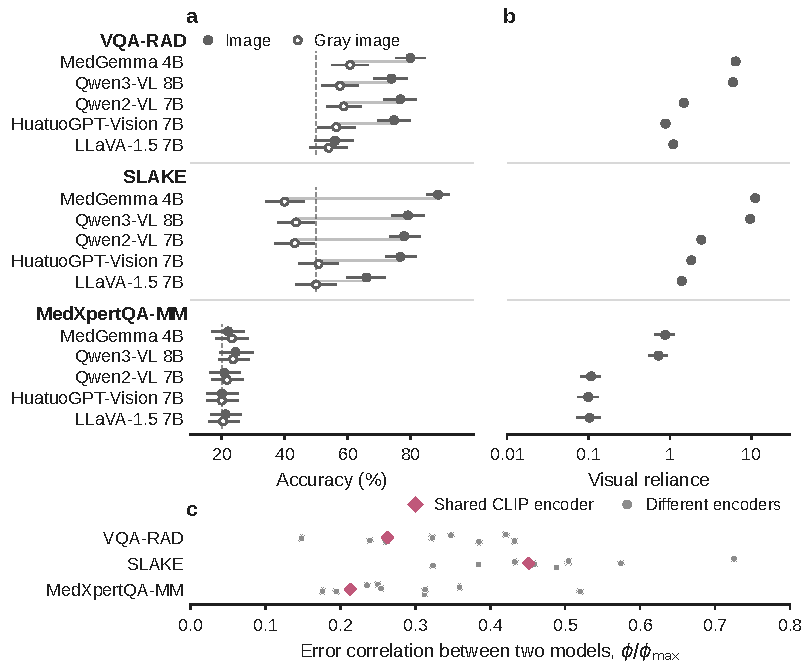
\includegraphics[width=\textwidth]{figures/fig_openweight.pdf}
\caption{Open-weight models, one forward pass per item. (a) Accuracy with the image (filled) and with a uniform gray image (open); dashed lines, chance. (b) Visual reliance: absolute change in the log-odds of ``yes'' between the image and the gray image on yes/no items, Kullback--Leibler divergence on MedXpertQA-MM; mean with item bootstrap 95\% CI, log scale. (c) Error correlation between two models divided by its maximum for their error rates ($\phi/\phi_{\max}$); diamonds, the pair that shares the CLIP ViT-L/14-336 vision encoder.}
\label{fig:openweight}
\end{figure}

\section*{S5. Text-only clinical questions}
The same reading-panel designs were applied to text-only clinical questions in a companion analysis: 8 language models from OpenAI, Google, Anthropic and DeepSeek answered items from MedQA, MedAgentsBench and the text set of MedXpertQA as single readers and as independent, centralized, discussion and tiered panels of 3 to 9 readers with specialty roles. Over 340 panel configurations, the first-round error correlation between panel positions was 0.758, which leaves 1.27 effective independent readers in a panel of 9. Over the 96 discussion configurations, discussion raised the error correlation from 0.758 (SD 0.117) to 0.990 (SD 0.010), or 1.01 effective readers. Error correlation and its rise during discussion therefore had the same magnitude without images as in the imaging experiments.

\end{document}
